%----------------------------------------------------------------------------------------
%	PACKAGES AND DOCUMENT CONFIGURATIONS
%----------------------------------------------------------------------------------------
\documentclass[article, a4paper, 12pt, oneside]{memoir}

% Margins
\usepackage[top=3cm,left=2cm,right=2cm,bottom=3cm]{geometry}

% Encondings
\usepackage[utf8]{inputenc}

% Language
\usepackage[portuguese]{babel}

% Graphics and images
\usepackage{graphicx}
	\graphicspath{{../images/}}

% Listings
\usepackage{listings}

% Color
\usepackage[dvipsnames]{xcolor}

% Tables
\usepackage{tabularx}

% Math symbols
\usepackage{amssymb}

% Paragraph Spacing
\usepackage{parskip}
\usepackage{indentfirst}
\setlength{\parskip}{0.5cm}

% Hyperreferences
\usepackage{hyperref}

% Repeated commands
\usepackage{expl3}
\ExplSyntaxOn
\cs_new_eq:NN \Repeat \prg_replicate:nn
\ExplSyntaxOff

% Header and Footer Things
\usepackage{wallpaper}
\usepackage{fancyhdr}

% Following code to edit the pagestyle
\pagestyle{fancy}
\fancyhf{}
\rhead{Meat Wagons}
\lhead{\leftmark}
\rfoot{Página \thepage}

% Commands
\usepackage{xargs}

%% Linked Email
\newcommand{\email}[1]{
{\texttt{\href{mailto:#1}{#1}} }
}

%----------------------------------------------------------------------------------------
%	DOCUMENT INFORMATION
%----------------------------------------------------------------------------------------
% Title
\title{\Huge \texttt{Meat Wagons - Transporte de Prisioneiros} }
% Authors
\author{
\LARGE \textbf{Turma 2 Grupo 3}\\\\
\begin{tabular}{l r}
	\email{up201806250@fe.up.pt} & Diogo Samuel Gonçalves Fernandes	\\
	\email{up201806490@fe.up.pt} & Hugo Miguel Monteiro Guimarães \\
	\email{up201806554@fe.up.pt} & Telmo Alexandre Espirito Santo Baptista	\\
\end{tabular}
}

%\institute{Faculdade de Engenharia da Universidade do Porto \\ Bases de Dados (BDAD) - Turma 4, grupo 6}

% Date for the report
\date{\today}

% Table of Contents
\addto\captionsportuguese{\renewcommand*\contentsname{Índice}}

%----------------------------------------------------------------------------------------
%	DOCUMENT
%----------------------------------------------------------------------------------------
\begin{document}
%----------------------------------------------------------------------------------------
%	Front Page
%----------------------------------------------------------------------------------------
% Title Author and Date
\maketitle

% More information for front page
\begin{center}
\textbf{Projeto CAL - 2019/20 - MIEIC}
\Repeat{2}{\linebreak}
\begin{tabular}{l r}
	\textbf{Professor das Aulas Práticas}: & \href{https://sigarra.up.pt/feup/pt/func_geral.formview?p_codigo=419241}{Rosaldo José Fernandes Rossetti}
\end{tabular}
\Repeat{4}{\linebreak}
% FEUP Logo

\includegraphics[scale=0.4]{FEUP-logo.jpg}

\end{center}

\newpage
% Header Image
\CenterWallPaper{0.1}{FEUP-logo.jpg}
\addtolength{\wpXoffset}{-7.5cm}
\addtolength{\wpYoffset}{13.8cm}

%----------------------------------------------------------------------------------------
%	TABLE OF CONTENTS
%----------------------------------------------------------------------------------------
\tableofcontents*

\newpage
%----------------------------------------------------------------------------------------
%	CHAPTER 1 - Descrição do Problema
%----------------------------------------------------------------------------------------
\chapter[Descrição do Problema][Descrição do Problema]{Descrição do Problema} \label{\thechapter}

Os transportes de prisioneiros entre diversos estabelecimentos como, por exemplo, as prisões, esquadras e tribunais são feitos utilizando veículos que se encontrem adaptados ao serviço. Estes veículos têm a necessidade de serem altamente resistentes uma vez que é necessário garantir que os prisioneiros não conseguem escapar.

Para este projeto, queremos optimizar o percurso dos veículos de forma a recolher e entregar os prisioneiros nos pontos de interesse. De modo a cumprir o pretendido, é possivel dividir nas seguintes fases:

\subsection{Primeira Iteração - Recolha de prisioneiros utilizando um único veículo}
	Inicialmente consideramos que só existe uma única camioneta para realizar todos os serviços.
	Com a primeira iteração pretende-se que apenas um veículo vá recolher os prisioneiros a uma dada localização, tendo em conta a urgência da situação. As situações que sejam mais exigentes serão respondidas primeiro pelos veículos.

	É importante notar que a recolha só pode ser efetuada se existirem caminhos que liguem todos os pontos de interesse, ou seja, o grafo necessita de ser conexo.

	Algumas vezes, obras nas vias públicas podem fazer com que certas zonas tornem-se inacessíveis, inviabilizando o acesso ao destino de alguns prisioneiros. Avalie a conectividade do grafo, a fim de identificar pontos de recolha e de entrega com pouca acessibilidade.

\subsection{Segunda Iteração - Recolha de prisioneiros utilizando vários veículos}
	Durante a segunda  fase vai-se ter em consideração o diverso número de veículos que a frota possui. Alguns veículos vão diferir de outras, tendo cada veículo uma determinada função. Vão existir veículos específicos para transportar prisioneiros até aos aeroportos e linhas de comboio.

\subsection{Terceira Iteração - Recolha seletiva de prisioneiros utilizando vários veículos}
	Na terceira e última iteração vamos ter em consideração não só o número de veículos disponíveis, como também o número de pedidos de transporte de prisioneiros que um veículo pode realizar num único serviço. Um único veículo pode sair da central e transportar vários prisioneiros, desde que o número de prisioneiros não ultrapasse a capacidade do veículo.


\newpage

%----------------------------------------------------------------------------------------
%	CHAPTER 2 - Formalização do Problema
%----------------------------------------------------------------------------------------
\chapter[Formalização do Problema][Formalização do Problema]{Formalização do Problema} \label{\thechapter}

\section{Dados de Entrada}

$C_i$ - sequência de veículos, sendo $C_i(i)$ o seu i-ésimo elemento. Cada veículo é caraterizado por:
\begin{itemize}
	\item $capacity$ - número de prisioneiros que pode transportar
	\item $type$ - tipo de veículo
\end{itemize}

$R_i$ - sequência de pedidos de transporte de prisioneiros, sendo $R_i(i)$ o seu i-ésimo elemento. Cada pedido é caraterizado por:
\begin{itemize}
	\item $pickup$ - local de recolha dos prisioneiros
	\item $dest$ - local de destino dos prisioneiros
	\item $numPris$ - número de prisioneiros a serem transportados
	\item $type$ - tipo de prisioneiros
	\item $p_d$ - peso da distância no trajeto a efetuar
	\item $p_t$ - peso do tempo no trajeto a efetuar
\end{itemize}

$G_i = (V_i, E_i)$ - grafo dirigido pesado, composto por:
\begin{itemize}
	\item $V$ - vértices, representando pontos da rede viária, com:
		\begin{itemize}
			\item $ID$ - Identificador único do vértice
			\item $D$ - Densidade populacional no vértice
			\item $Adj \subseteq E$ - arestas que saiem do vértice
			\item $avg-speed$ - velocidade média na área em volta do vértice
			\item $reachable$ - se o vértice é alcançável a partir da central
		\end{itemize}
	\item $E$ - arestas, representando conexão entre dois pontos da rede viária, com:
		\begin{itemize}
			\item $ID$ - Identificador único da aresta
			\item $W_d$ - peso da aresta em relação à distância (representa a distância entre os dois vértices)
			\item $W_t$ - peso da aresta em relação ao tempo (representa o tempo médio que demora a percorrer a distância entre os dois vértices, considerando o tráfego normal naquela conexão da rede viária)
			\item $open$ - se a conexão entre os vértices está aberta, isto é, se a rua estiver cortada por alguma razão então não é possível utilizar esta conexão
		\end{itemize}
\end{itemize}

$S$ - vértice da central

\section{Dados de Saída}

$G_f = (V_f, E_f)$ - grafo dirigido pesado, tendo $V_f$ e $E_f$ os mesmos atributos que $V_i$ e $E_i$, excluindo atributos específicos do algoritmo utilizado

$C_f$ - sequência de veículos com os serviços a realizar, sendo $C_f(i)$ o seu i-ésimo elemento. Cada veículo é caraterizado por:
\begin{itemize}
	\item $S$ - sequência de serviços a realizar, sendo $S(i)$ o seu i-ésimo elemento. Cada serviço é caraterizado por:
	\begin{itemize}
		\item $emptySeats$ - número de lugares vazios
		\item $R_f$ - sequência de pedidos atendidos, sendo $R_f(i)$ o seu i-ésimo elemento. Cada pedido atendido é caraterizado por:
		\begin{itemize}
			\item $pickupHour$ - hora de chegada ao local de recolha
			\item $destHour$ - hora de chegada ao local de destino
			\item $p_d$ - peso da distância no trajeto a efetuar
			\item $p_t$ - peso do tempo no trajeto a efetuar
		\end{itemize}
		\item $P = { e ~ \in ~ E_i }$ - sequência de arestas a percorrer, sendo $P(i)$ o seu i-ésimo elemento
		\item $dist$ - distância percorrida no serviço
		\item $startHour$ - hora esperada de ínicio do serviço
		\item $endHour$ - hora esperada de termino do serviço
	\end{itemize}
\end{itemize}

\section{Restrições}

\subsection{Sobre os dados de entrada}

\begin{itemize}
	\item $\forall i ~ \in ~ [0, \vert C_i \vert [: capacity(C_i(i)) > 0$, uma vez que não faz sentido os veículos não poderem transportar prisioneiros
	\item $\forall r ~ \in ~ R_i, dest(r)$ deve pertencer ao mesmo componente fortemente conexo do grafo $G_i$ que o vértice $S$, uma vez que o veículo tem de ser capaz de voltar à central
	\item $\forall r ~ \in ~ R_i, numPris(r) > 0$, uma vez que não faz sentido ter um pedido para transportar zero prisioneiros
	\item $\forall r ~ \in ~ R_i, p_d \geq 0 \wedge p_t \geq 0 \wedge (p_d \neq 0 \vee p_t \neq 0)$
	\item $\forall v ~ \in ~ V_i, avg$-$speed(v) > 0$
	\item $\forall e ~ \in ~ E_i, W_d(e) > 0 \wedge W_t(e) > 0$, uma vez que o peso da aresta representa a distância ou o tempo médio necessário para percorrer a aresta, se esta distância ou tempo forem zero estaremos num ciclo no mesmo vértice
	\item $\forall e ~ \in ~ E_i, e$ deve ser uma rua ao qual os veículos possam utilizar, ruas que os veículos não tenham permissão para entrar não são incluídas no grafo $G_i$
	\item $S ~ \in ~ V_i$, uma vez que a central é um vértice do grafo $G_i$
\end{itemize}

\subsection{Sobre os dados de saída}

\begin{itemize}
	\item $\vert C_f \vert \leq \vert C_i \vert $ - não se pode usar mais veículos que os disponíveis
	\item $\forall v_f ~ \in ~ V_f, \exists v_i ~ \in ~ V_i$ tal que $v_i$ e $v_f$ têm os mesmos valores para todos os atributos, com exceção de atributos especificos aos algoritmos utilizados
	\item $\forall e_f ~ \in ~ E_f, \exists e_i ~ \in ~ E_i$ tal que $e_i$ e $e_f$ têm os mesmo valores para todos os atributos, com exceção de atributos especificos aos algoritmos utilizados
	\item $\forall r_f ~ \in ~ R_f, \exists r_i ~ \in ~ R_i$ tal que $r_f$ e $r_i$ têm os mesmo valores para os atributos $p_d$ e $p_t$
	\item $\forall c ~ \in ~ C_f, \forall s ~ \in ~ S(c), 0 \leq emptySeats < capacity(c)$ pois cada serviço deve ter pelo menos um prisioneiro, e não pode haver sobrelotação do veículo
	\item $\forall c ~ \in ~ C_f, \forall s ~ \in ~ S(c), \vert R_f(s) \vert > 0$ uma vez que só faz sentido realizar um serviço se for houver um pedido de transporte de prisioneiros
	\item $\forall c ~ \in ~ C_f, \forall s ~ \in ~ S(c), endHour(s) > startHour(s)$
	\item $\forall c ~ \in ~ C_f, \forall s ~ \in ~ S(c), startHour(s) < pickupHour(\forall r ~ \in ~ R_f) < endHour(s) ~ \wedge ~ startHour(s) < destHour(\forall r ~ \in ~ R_f) \leq endHour(s)$
\end{itemize}

\section{Função objetivo}

A solução ótima passa por minizar a soma ponderada da distância percorrida e o tempo do serviço de um determinado veículo, que resulta na seguinte função:

$\sum_{c ~ \in ~ C_f} \sum_{s ~ \in ~ S} \sum_{e ~ \in ~ P} (W_d(e) * max(p_d(R_f(s))) + W_t(e) * max(p_t(R_f(s))$

\begin{itemize}
	\item $max(p_d(R_f(s))$ - é o maior valor para o peso da distância numa determinada sequência de pedidos de um serviço de um veículo 
	\item $max(p_t(R_f(s))$ - é o maior valor para o peso do tempo numa determinada sequência de pedidos de um serviço de um veículo
\end{itemize}

Deste modo, obtivemos a função objetivo para o nosso problema que se encontra acima.

\newpage
%----------------------------------------------------------------------------------------
%	CHAPTER 3 - Perspectiva de solução
%----------------------------------------------------------------------------------------
\chapter[Perspectiva de solução][Perspectiva de solução]{Perspectiva de solução} \label{\thechapter}

\section{Pré-processamento dos dados de entrada}

\subsection{Grafo}
Partindo da central todos os vértices que não forem alcançáveis têm a variável $reachable$ definida como falsa.

Além disso, todas os vértices do grafo que não pertençam à componente fortemente conexa de origem devem ser marcados como inacessíveis ($reachable$ é colocado a falso).

\subsection{Pedidos de transporte de prisioneiros}
Remover todos os pedidos de transporte de prisioneiros que não pertençam ao grafo pré-processado, isto é, remover aqueles que façam parte de arestas que têm a componente $open$ definida como falsa.

Também devemos organizar os pedidos de transporte de prisioneiros por ordem decrescente do número de prisioneiros a transportar, facilitando depois no alocamento de veículos para o seu transporte.

\subsection{Veículos para transporte de prisioneiros}
Relativamente ao pré-processamento dos veículos de transporte, devemos organizá-los por ordem decrescente de capacidade. Assim, como também temos os pedidos de transporte de prisioneiros organizados por ordem decrescente do número de prisioneiros a transportar podemos potencialmente minizar o número de veículos utilizados.

\section{Identificação do problema}

A empresa de transporte de prisioneiros Meat Wagons necessita de transportar os prisioneiros  de um ponto de recolha até um determinado destino. De modo a otimizar este transporte, a empresa optou por procurar o caminho mais eficiente para a efetuar a viagem. 

Na primeira iteração, onde apenas está disponível um veículo, que realiza os pedidos de transporte um de cada vez, este problema trata-se do \textbf{caminho mais curto} entre a origem e o local de recolha seguido do \textbf{caminho mais curto} entre o local de recolha e o destino. A segunda iteração é semelhante à primeira iteração, variando apenas o número de veículos disponíveis para realizar os pedidos.

Na terceira e última iteração, não só varia o número de veículos disponíveis, como também o número de pedidos de transporte que um veículo pode realizar num único serviço, equiparando-se ao problema designado por \textbf{Vehicle Routing Problem}, uma generalização do problema do \textbf{Travelling Salesman Problem}, um problema NP-díficil.

Vale também realçar que os veículos devem retornar para a central no fim 

\section{Caminho mais curto}
Este é o problema referido na primeira e segunda iteração, e trata-se de encontrar o percurso mais curto e eficiente entre dois pontos, ou entre todos os pares de pontos do grafo.

\subsection{Entre dois pontos}
Entre os vários algoritmos que existem para calcular o caminho mais curto entre dois pontos destacam-se os seguintes algoritmos:

\subsubsection{Algoritmo de Dijkstra}
Este algoritmo foi concebido por \href{https://en.wikipedia.org/wiki/Edsger_W._Dijkstra}{Edsger W. Dijkstra} e resolve problemas do caminho mais curto de uma única origem em grafos que possuam pesos não negativos.

Para poder aplicar este algoritmo é necessário que cada vértice guarde a seguinte informação:
\begin{itemize}
	\item $W$ - custo mínimo até ao local da origem (combinação linear da distância e tempo, como visto na função objetivo)
	\item $path$ - vértice antecessor no caminho mais curto
\end{itemize}

O algoritmo de Dijkstra pode utilizar uma $priority queue$ ou um $array$ para inserir os novos vértices. 
Este consiste em inicializar os vértices, o que se pode fazer em tempo linear $O(|V|)$. Seguidamente, inicializar a estrutura auxiliar, que neste caso consideramos a $priority queue$ devido a ter maior eficiência relativamente ao $array$, com o vértice origem.

Processam os vértices que se encontram na queue extraindo-os e seguidamente percorrendo cada aresta do vértice a ser processado. Posteriormente, se o custo relativo ao vértice de destino da aresta for maior do que o custo do caminho atual, terá que se atualizar o vértice de destino e inserindo na $priority queue$ caso ele ainda não esteja na fila de processamento ou fazendo a operação $DECREASE-KEY$ caso este já esteja na fila de processamento.

As operações de inserção, extração e $DECREASE-KEY$ têm complexidade temporal $O(log(N))$. Dado que é necessário percorrer todos os vértices e arestas resulta numa complexidade de $O((|V| + |E|)*log(|V|))$.

Assim podemos concluir que o tempo de execução do algoritmo é $O((|V| + |E|)*log(|V|))$.

O pseudo-código para implementar este algoritmo é o seguinte:

\begin{lstlisting}[frame=single, mathescape=true]
FOR EACH v $\in$ V DO
  COST(v) $\leftarrow$ $\infty$
  PATH(v) $\leftarrow$ NULL

COST(s) $\leftarrow$ 0
Q $\leftarrow$ $\varnothing$ // MIN PRIORITY QUEUE
INSERT(Q, (s, COST(s)))
WHILE Q $\neq$ $\varnothing$ DO
  v $\leftarrow$ EXTRACT-MIN(Q)
  FOR EACH w $\in$ Adj(v) DO
    IF COST(w) > COST(v) + WEIGHT(v, w) THEN
      COST(w) $\leftarrow$ COST(v) + WEIGHT(v, w)
      PATH(w) $\leftarrow$ v
      IF w $\notin$ Q THEN
        INSERT(Q, (w, COST(w)))
      ELSE
        DECREASE-KEY(Q, (w, COST(w)))
\end{lstlisting}

Este algoritmo destaca-se pela sua facilidade de implementação, porém o algoritmo pode explorar demasiados vértices desnecessários.

A ineficiência do algoritmo pode ser visto na imagem abaixo:

\begin{figure}[h]
\centering
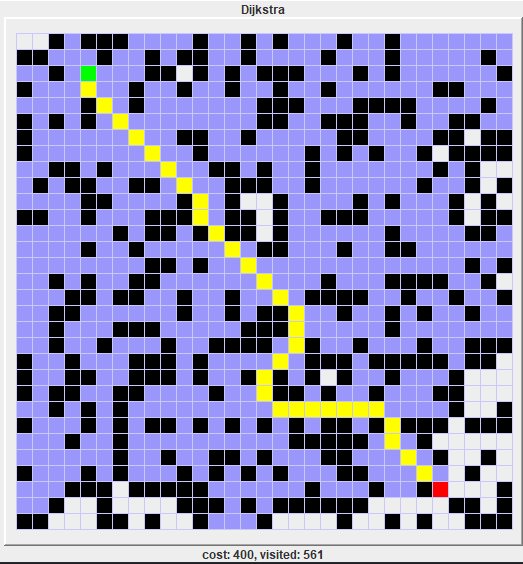
\includegraphics[scale=0.4]{dijkstra}
\caption{\emph{Dijkstra's algorithm}}
\begin{tabular}{ l r }
\color{black} $\blacksquare$ \color{black} walls & \color{Periwinkle} $\blacksquare$ \color{black} visited \\
\color{green} $\blacksquare$ \color{black} origin & \color{red} $\blacksquare$ \color{black} destination \\
\color{yellow} $\blacksquare$ \color{black} shortest path
\end{tabular}
\end{figure}

\subsubsection{Algoritmo de Bellman-Ford}
O algoritmo de Bellman-Ford corresponde a uma extensão do algoritmo de Dijkstra permitindo a existência de pesos negativos nas arestas, sendo mais lento que o de Dijkstra por esse mesmo motivo.

Uma vez que foi imposta a restrição de pesos não negativos nas arestas, este algoritmo não se vê útil, uma vez que não se vê necessário tratar pesos negativos.

\subsubsection{Algoritmo A*}
O algoritmo A*, desenvolvido por \href{https://en.wikipedia.org/wiki/Peter_E._Hart}{Peter Hart}, \href{https://en.wikipedia.org/wiki/Nils_John_Nilsson}{Nils Nilsson} e \href{https://en.wikipedia.org/wiki/Bertram_Raphael}{Bertram Raphael}, pode ser visto como uma extensão do algoritmo de Dijkstra, usando heurística para guiar a sua pesquisa.

Em cada iteração, o algoritmo precisa decidir qual caminho processar, baseando-se no custo  do caminho desde a origem até ao ponto atual e numa estimativa do custo do caminho desde o vértice adjacente a testar até ao destino, isto é o algoritmo visa minimizar a seguinte função
\begin{equation}
f(n) = g(n) + h(n)
\end{equation}
onde $n$ é o próximo vértice do caminho, $g(n)$ o custo desde a origem até $n$ e $h(n)$ uma estimativa do custo mínimo desde $n$ até ao destino.

Uma possível implementação do algoritmo está demonstrada no seguinte pseudo-código:
\begin{lstlisting}[frame=single, mathescape=true]
RECONSTRUCT_PATH(current)
  path $\leftarrow$ {current}
  WHILE PATH(current) $\neq$ NULL
    current $\leftarrow$ PATH(current)
    path.PUSH_FRONT(current)
  RETURN path

A_STAR(start, goal, heuristic)
  FOR EACH v $\in$ V DO
    G_COST(v) $\leftarrow$ $\infty$
    F_COST(v) $\leftarrow$ $\infty$
    PATH(v) $\leftarrow$ NULL

  G_COST(start) $\leftarrow$ 0
  F_COST(start) $\leftarrow$ heuristic(start) // G_COST(start)+heuristic(start)
  Q $\leftarrow$ $\varnothing$ // MIN PRIORITY QUEUE
  INSERT(Q, (start, COST(start)))
  WHILE Q $\neq$ $\varnothing$ DO
    v $\leftarrow$ EXTRACT-MIN(Q)	
    IF V = GOAL
      RETURN RECONSTRUCT_PATH(v)
    
    FOR EACH w $\in$ Adj(v) DO
      IF G_COST(w) > G_COST(V) + WEIGHT(v, w) THEN
        G_COST(w) $\leftarrow$ G_COST(v) + WEIGHT(v, w)
        PATH(w) $\leftarrow$ v
        F_COST(w) $\leftarrow$ G_COST(w) + heuristic(w)
        IF w $\notin$ Q THEN
          INSERT(Q, (w, COST(w)))
        ELSE
          DECREASE-KEY(Q, (w, COST(w)))
\end{lstlisting}

O algoritmo A* é um algoritmo de elevada eficiência e otimização, sendo usado em muitos contextos, como nos sistemas de \href{https://en.wikipedia.org/wiki/Journey_planner}{encaminhamento de viagens} que corresponde às duas primeiras iterações do nosso problema.

A eficiência deste algoritmo pode ser observada comparando o número de vértices explorados durante a pesquisa com o algoritmo de Dijkstra, como é demonstrado na imagem abaixo:

\begin{figure}[h]
\centering
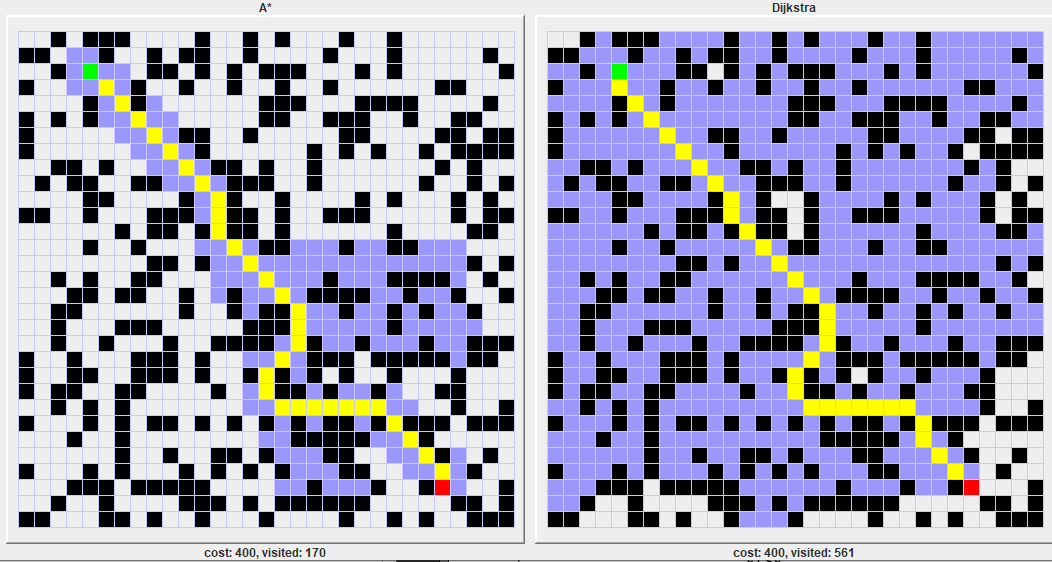
\includegraphics[scale=0.4]{pathfinder}
\caption{\emph{A* algorithm \textbf{vs.} Dijkstra's algorithm}}
\begin{tabular}{ l r }
\color{black} $\blacksquare$ \color{black} walls & \color{Periwinkle} $\blacksquare$ \color{black} visited \\
\color{green} $\blacksquare$ \color{black} origin & \color{red} $\blacksquare$ \color{black} destination \\
\color{yellow} $\blacksquare$ \color{black} shortest path
\end{tabular}
\end{figure}

Embora a eficiência do algoritmo seja maior, o algoritmo A* não garante a solução ótima para todos os casos, ao contrário de algoritmos como o de Dijkstra. Esta desvantagem pode ser observada na imagem abaixo:

\begin{figure}[h]
\centering
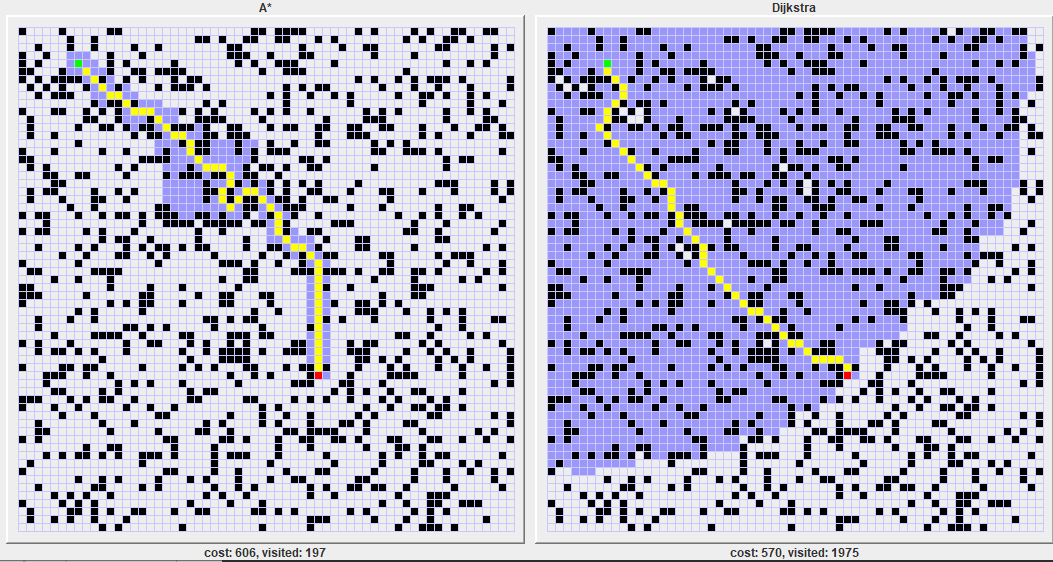
\includegraphics[scale=0.4]{pathfinder2}
\caption{\emph{A* algorithm \textbf{vs.} Dijkstra's algorithm}}
\begin{tabular}{ l r }
\color{black} $\blacksquare$ \color{black} walls & \color{Periwinkle} $\blacksquare$ \color{black} visited \\
\color{green} $\blacksquare$ \color{black} origin & \color{red} $\blacksquare$ \color{black} destination \\
\color{yellow} $\blacksquare$ \color{black} shortest path
\end{tabular}
\end{figure}

Analisando os resultados obtidos, é possível constatar que o algoritmo de Dijkstra visitou aproxidamente dez vezes mais vértices que o algoritmo A* ($1975 ~ \textbf{vs.} ~ 197$). Porém, o caminho mais curto encontrado pelo algoritmo A* não corresponde ao caminho com menor custo, uma vez que o caminho encontrado pelo algoritmo de Dijkstra possui um custo menor que o algoritmo de A* ($570 ~ \textbf{vs.} ~ 606$).

\subsection{Entre todos os pares de vértices}
É possível calcular o caminho entre todos os pares de vértices através de algoritmos, como a aplicação repetida do algoritmo de Dijkstra ou a utilização do algoritmo de Floyd-Warshall.

Estes algoritmos são bastante utilizados para pré-processamento de mapas de estradas, porém no nosso problema, como os pesos para a distância e o para o tempo variam de pedido para pedido, o pré-processamento dos caminhos mais curtos para todos os pares de vértices não traria nenhuma vantagem, apenas uma diminuição na eficiência do programa.

\section{Caminho mais curto com vários pedidos}
Dada a possibilidade de um veículo realizar vários pedidos num único serviço, existirá um conjunto de locais de recolha e locais de destino a serem percorridos.

Deparamo-nos então com um problema similar ao \textbf{Travelling Salesman Problem}, um problema NP-díficil. Como se trata de um grafo dirigido é a versão assimétrica do problema \textbf{Travelling Salesman Problem}

As soluções deste problema podem dividir-se em duas categorias:
\begin{itemize}
	\item \textbf{Soluções Exatas} - algoritmos que encontram a solução exata do problema
	\item \textbf{Soluções Aproximadas} - algoritmos que aproximam a solução do problema através de heurísticas e aproximações
\end{itemize}

\subsection{Soluções Exatas}
\subsubsection{Brute-force}
O método brute-force testa todas as permutações possíveis para o percurso, atualizando o caminho ótimo sempre que encontra um custo menor ao atual, resultando assim numa complexidade $O(n!)$, sendo $n$ o número de vértices a percorrer.

\subsubsection{Held-Karp}

\begin{lstlisting}[frame=single, mathescape=true]
FALTA EXPLICAR + PSEUDo
\end{lstlisting}

Analisando as complexidades dos algoritmos apresentados podemos verificar que o método de brute-force é mais eficiente para valores de $n$ menores que sete, sendo o algoritmo de Held-Karp mais eficiente para os restantes valores de $n$, sendo $n$ o número de vértices a percorrer, assim como se pode observar no gráfico seguinte:

\begin{figure}
\centering
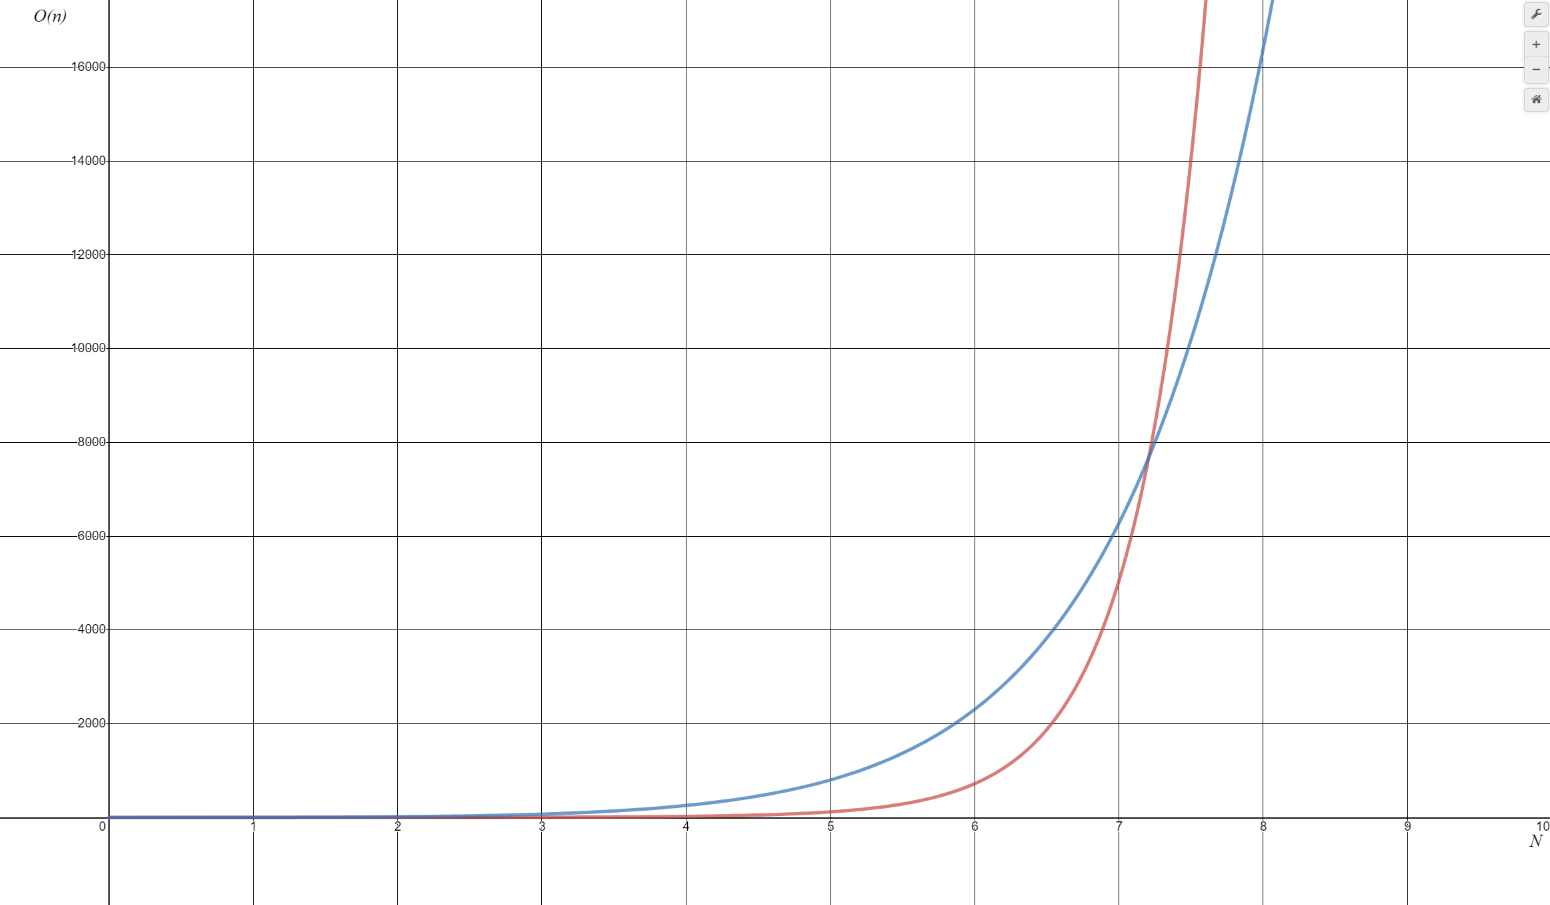
\includegraphics[scale=0.3]{tsp_exact_complexity}
\caption{\emph{Brute-force \textbf{vs.} Held-Karp algorithm: Complexities}}
\begin{tabular}{ l r }
\color{red} $-$ \color{black} Brute-force ($O(n!)$) & \color{blue} $-$ \color{black} Held-Karp ($O(n^22^n)$)
\end{tabular}
\end{figure}

Na implementação do cálculo da solução exata alternaríamos o método utilizado conforme o número de vértices a percorrer, usando brute-force para $n \leq 7$ e o algoritmo Held-Karp para $n > 7$. 

\subsection{Soluções Aproximadas}
\subsubsection{Nearest Neighbour}
O algoritmo de \textbf{nearest neighbour} consiste em escolher um vértice aleatório para o ínicio, e de seguida escolher o vértice mais próximo como próximo vértice a percorrer repetindo este passo até visitar todos os vértices a serem percorridos. Trata-se assim de algoritmo ganancioso que encontra uma solução aproximada em tempo reduzido, no entanto esta solução não é garantidamente a solução ótima.

O pseudo-código deste algoritmo é o seguinte:
\begin{lstlisting}[frame=single, mathescape=true]
FOR EACH v \in V DO
  VISITED(v) $\leftarrow$ false
  PATH(v) $\leftarrow$ NULL

v $\leftarrow$ RANDOM_VERTEX(V) // choose starting point
VISITED(v) $\leftarrow$ true

WHILE NOT ALL_VISITED(V) DO
  w $\leftarrow$ CLOSEST_VERTEX(V, v) // get closest vertex to v
  VISITED(w) $\leftarrow$ v 
  PATH(w) $\leftarrow$ v
  v $\leftarrow$ w
\end{lstlisting}

\subsubsection{Algoritmo Genético}
Algoritmos genéticos são algoritmos baseados em heurísticas que simulam o processo de evolução de espécies, o processo de \href{https://en.wikipedia.org/wiki/Natural_selection}{\emph{seleção natural}}, selecionando os melhores espécimes de cada geração.

Os algoritmos genéticos podem ser divididos em cinco fases:
\begin{enumerate}
	\item Gerar a população
	\item Calcular a aptidão de cada indivíduo da população
	\item Escolher os indivíduos mais aptos
	\item Reproduzir os indivíduos escolhidos (por replicação ou \emph{crossover})
	\item Mutação dos indivíduos de modo a introduzir pequenas variações na população
\end{enumerate}

\begin{lstlisting}[frame=single, mathescape=true]
// calculate  fitness
CALCULATE_FITNESS(I)
  fitness $\leftarrow$ 0
  FOR i $\leftarrow$ 1 TO $\vert VERTICES(I) \vert$
    // add cost of going from vertex i-1 to vertex i
    fitness $\leftarrow$ fitness + COST(VERTICES[i-1], VERTICES[i])
  FITNESS(I) $\leftarrow$ fitness

// Choose the n best individuals
CULL_POPULATION(P, n)
  sorted $\leftarrow$ SORT_BY_FITNESS(P) // sort by descending order of fitness
  best $\leftarrow$ $\varnothing$
  FOR i $\leftarrow$ 0 TO n
    INSERT(best, sorted(i))
  RETURN best

// replicate individual
REPLICATE(I)
  return EXACT_COPY(I)
  
// create new individual from two parents
CROSSOVER(parent_A, parent_B)
  child $\leftarrow$ NEW_INDIVIDUAL()
  // being N the number of vertices to visit
  // random integer in [0, N[
  section_start $\leftarrow$ RANDOM_INT(0, N)
  // random integer in ]section_start, N[
  section_end $\leftarrow$ RANDOM_INT(section_start + 1, N)
  // copy random section from parent A
  FOR i $\leftarrow$ section_start TO section_end DO
    VERTICES(child) AT (i) $\leftarrow$ VERTICES(parent_A) AT (i)
  
  // fill remaining empty sections with genes from parent B
  FOR i $\leftarrow$ 0 TO N DO
    IF VERTICES(child) AT (i) = NULL
      VERTICES(child) AT (i) $\leftarrow$ VERTICES(parent_B) AT (i)
  RETURN CHILD

// mutate individual
MUTATE(I)
  v $\leftarrow$ RANDOM_VERTEX(VERTICES(I)) // choose random vertex
  w $\leftarrow$ RANDOM_VERTEX(VERTICES(I)) // choose another random vertex
  SWAP(v, w)

// using crossover to reproduce (can be done with replication)
// reproduces population P
REPRODUCE_POPULATION(P)
  NEW_P $\leftarrow$ $\varnothing$
  FOR i $\leftarrow$ 0 TO POPULATION_SIZE DO
    // choose parents (can be tested to be different parents)
    parent_A $\leftarrow$ RANDOM_INDIVIDUAL(P)
    parent_B $\leftarrow$ RANDOM_INDIVIDUAL(P)
    I $\leftarrow$ CROSSOVER(parent_A, parent_B)
    random $\leftarrow$ RANDOM_FLOAT(0, 1) // random number between 0 and 1
    IF random < MUTATION_RATE THEN
      MUTATE(I)
    INSERT(NEW_P, I)
  RETURN NEW_P
  

// generate random population (random order of vertices to visit)
P $\leftarrow$ GENERATE_RANDOM_POPULATION(V)

WHILE ... // decide stopping criteria
  FOR EACH individual $\in$ P
    CALCULATE_FITNESS(individual)
  
  best $\leftarrow$ CULL_POPULATION(P, n)
  P $\leftarrow$ REPRODUCE_POPULATION(best) // reproduce best individuals
\end{lstlisting}

%----------------------------------------------------------------------------------------
%	CHAPTER 3 - Funcionalidades a implementar
%----------------------------------------------------------------------------------------
\chapter[Funcionalidades a implementar][Funcionalidades a implementar]{Funcionalidades a implementar} \label{\thechapter}

\section{Pré-processamento dos dados de entrada}

\subsection{Grafo}
De modo a marcar todas as arestas alcançáveis a partir do vértice da central pode ser utilizada uma estratégia semelhante à procura em profundidade ($Depth-First Search$), começando a visita na central, e marcar todos os vértices que forem visitados como $open$.

O pseudo-código para esta estratégia é o seguinte:

\begin{lstlisting}[frame=single, mathescape=true]
VISIT(node)
  reachable(node) $\leftarrow$ true
  FOR w $\in$ Adj(node) DO
    IF NOT reachable(w) THEN
      VISIT(w)

// G - graph
// source - starting point
VISIT_FROM_SOURCE(G, source)
  FOR v $\in$ VERTICES(G) DO
    reachable(v) $\leftarrow$ false

  VISIT(source)
\end{lstlisting}

Para a identificação dos vértices do grafo que pertençam à componente fortemente conexa do vértice da central, será necessário analisar a conetividade do grafo e a construção do componente fortemente conexo, para o qual se destacam os algoritmos de Kosaraju e de Tarjan.

\subsubsection{Algoritmo de Kosaraju}

\begin{lstlisting}[frame=single, mathescape=true]
// S - stack to store vertices in post order
DFS_VISIT(node, S)
  visited(node) $\leftarrow$ true
  FOR w $\in$ Adj(v) DO
    IF not visited(w) THEN
      DFS_VISIT(w)
  INSERT(S, node)

// get strongly connected component of vertex source
GET_SCC(G, source)
  S $\leftarrow$ $\varnothing$ // empty stack

  DFS_VISIT(source)

  GT $\leftarrow$ TRANSPOSE(G)
  
\end{lstlisting}

ACABAR ISTO AQUI


\section{Casos de Implementação}

Perante a organização dos caminhos a percorrer pelos veículos, é necessário ter em consideração os seguintes aspetos:

- Escolha do melhor percurso para um veículo;
- Escolha dos pedidos de transporte de prisioneiros para cada veículo

- Agrupar os pedidos de prisioneiros;
- Agrupamento dos veículos;

Deve ter-se como objetivo a atribuição de uma carrinha a um serviço, tendo atenção aos prisioneiros que se precisam de transportar.

É necessário ter em consideração a urgência do transporte de um prisioneiro, pelo que se devem agrupar os prisioneiros cujos locais de partida e chegada sejam pouco distantes, priorizando sempre o transporte dos prisioneiros mais urgentes.

Devem ser, portanto, seguidos os seguintes passos quando é recebido um novo pedido de transporte de prisioneiros:

- Ordenação dos serviços de modo a que os pedidos de transporte de prisioneiros mais recentes sejam analisados primeiro.  

- Escolha do veículo disponível que possa efetuar os pedidos que foram recebidos num determinado período de tempo.

- Verificar se veículos que estão a executar algum pedido estão aptos à existência de novos pedidos de transporte de prisioneiros. Se um veículo puder efetuar esse pedido sem alterar o seu percurso, então o pedido deve ser sempre aceite.



\newpage
\chapter{Bibliografia}
\begin{itemize}
	\item Apresentações fornecidas pelo professor Rosaldo José Fernandes Rossetti nas aulas téoricas da cadeira \href{https://sigarra.up.pt/feup/pt/ucurr_geral.ficha_uc_view?pv_ocorrencia_id=436441}{Conceção e Análise de Algoritmos}
	\item \color{blue} \underline{\href{https://en.wikipedia.org/wiki/Shortest_path_problem}{Shortest Path Problem}} \color{black}
	\item \color{blue} \underline{\href{https://en.wikipedia.org/wiki/Dijkstra\%27s_algorithm}{Dijkstra's Algorithm}} \color{black}
	\item \color{blue} \underline{\href{https://en.wikipedia.org/wiki/Bellman\%E2\%80\%93Ford_algorithm}{Bellman-Ford Algorithm}} \color{black}
	\item \color{blue} \underline{\href{https://en.wikipedia.org/wiki/A*_search_algorithm}{A* algorithm}} \color{black}
	\item \color{blue} \underline{\href{https://en.wikipedia.org/wiki/Admissible_heuristic}{Admissible heuristic}} \color{black}
	\item \color{blue} \underline{\href{https://en.wikipedia.org/wiki/Travelling_salesman_problem}{Traveling Salesman Problem}} \color{black}
	\item \color{blue} \underline{\href{https://en.wikipedia.org/wiki/Vehicle_routing_problem}{Vehicle Routing Problem}} \color{black}
	\item \color{blue} \underline{\href{https://en.wikipedia.org/wiki/Held\%E2\%80\%93Karp_algorithm}{Held-Karp algorithm}} \color{black}
	\item \color{blue} \underline{\href{https://en.wikipedia.org/wiki/Nearest_neighbour_algorithm}{Nearest neighbour algorithm}} \color{black}
	\item \color{blue} \underline{\href{https://en.wikipedia.org/wiki/Genetic_algorithm}{Genetic Algorithm}} \color{black}
	\item \color{blue} \underline{\href{https://en.wikipedia.org/wiki/Natural_selection}{Natural selection}} \color{black}
	\item \color{blue} \underline{\href{https://en.wikipedia.org/wiki/DNA_replication}{DNA replication}} \color{black}
	\item \color{blue} \underline{\href{https://en.wikipedia.org/wiki/Chromosomal_crossover}{Chromosomal crossover}} \color{black}
	\item \color{blue} \underline{\href{https://en.wikipedia.org/wiki/Mutation}{Mutation}} \color{black}
	\item \color{blue} \underline{\href{https://www.geeksforgeeks.org/strongly-connected-components}{GeeksForGeeks - Strongly connected components}} \color{black}
	\item \color{blue} \underline{\href{https://en.wikipedia.org/wiki/Kosaraju\%27s_algorithm}{Kosaraju's algorithm}} \color{black}
	\item \color{blue} \underline{\href{https://en.wikipedia.org/wiki/Tarjan\%27s_strongly_connected_components_algorithm}{Tarjan's algorithm}} \color{black}
	\item \color{blue} \underline{\href{https://www.geeksforgeeks.org/tarjan-algorithm-find-strongly-connected-components}{GeeksForGeeks - Tarjan's algorithm}} \color{black}
	\item \color{blue} \underline{\href{https://www.desmos.com/calculator}{Desmos Graphing Tool}} \color{black}
	\item \color{blue} \underline{\href{https://github.com/kevinwang1975/PathFinder}{Path Finder Visualization Program}} \color{black}
\end{itemize}

\end{document}
